% \subsubsection{Hướng dẫn sử dụng}
% 	\begin{figure}[H]
% 		\centering
% 		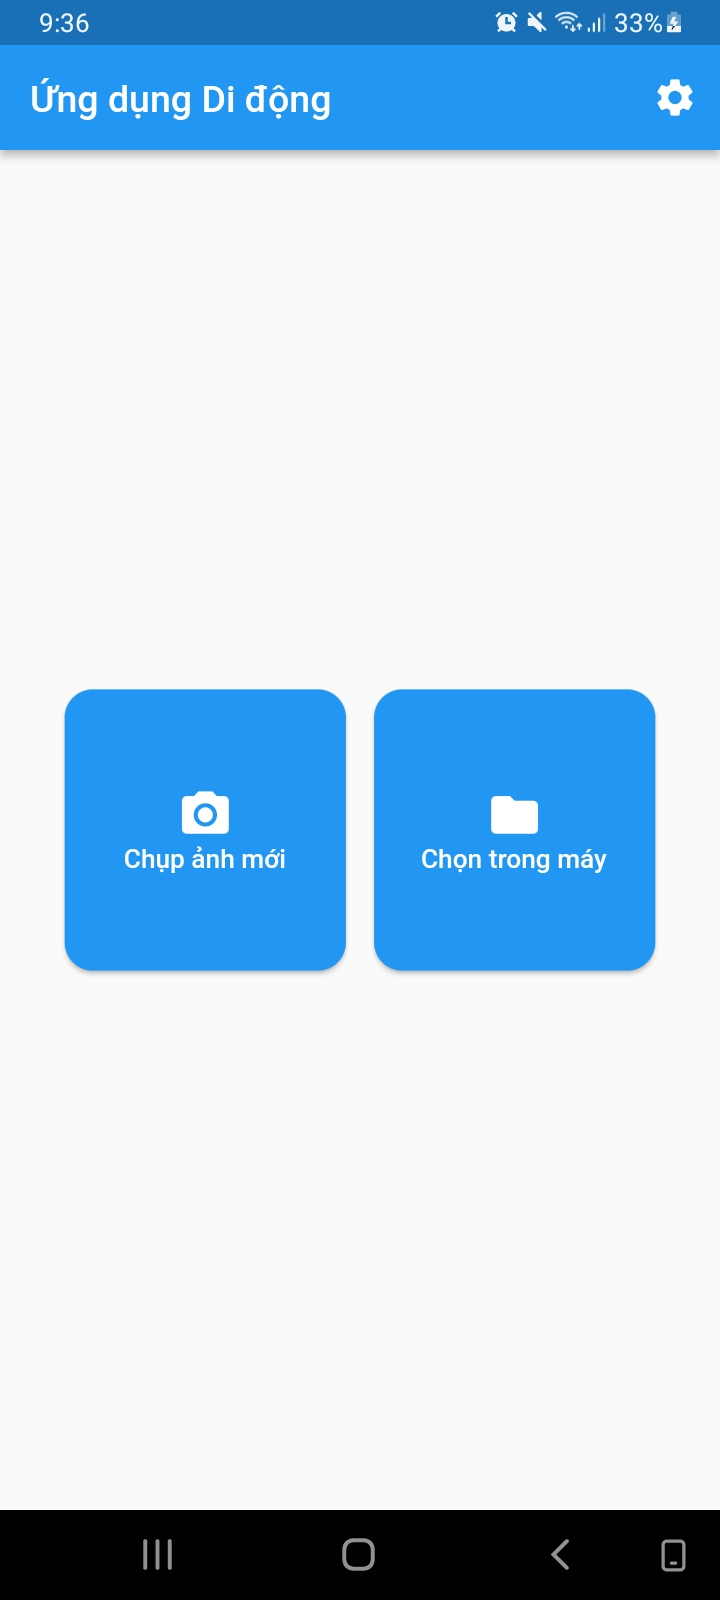
\includegraphics[scale=0.1]{images/screenshot1.jpg}
% 		\caption{Màn hình chính}
% 	\end{figure}

% 	Ở màn hình chính, có 2 lựa chọn: \textbf{Chụp ảnh mới} (chụp ảnh từ camera để lấy ảnh) và \textbf{Chọn trong máy} (chọn ảnh có sẵn trong bộ nhớ của máy).

% 	\begin{figure}[H]
% 		\centering
% 		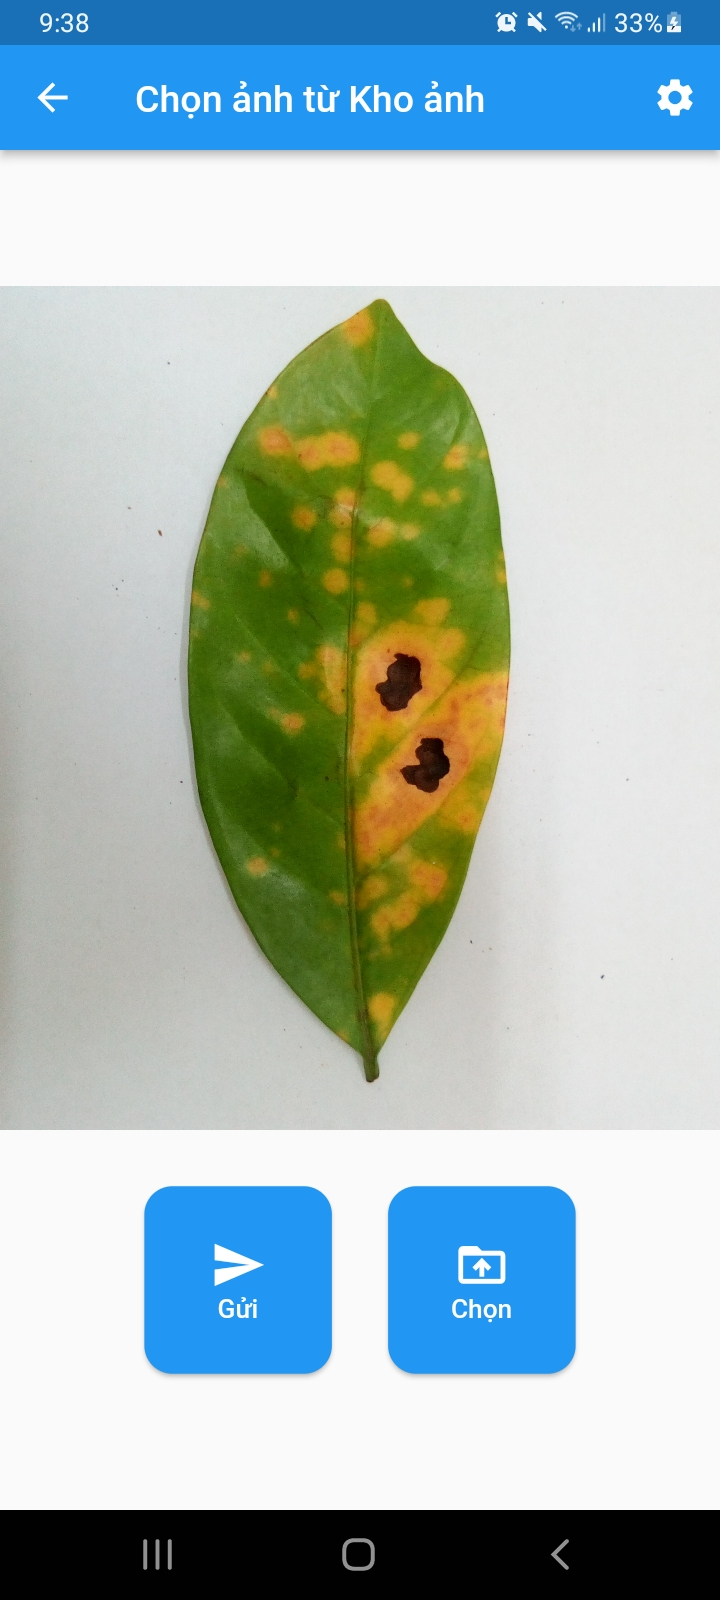
\includegraphics[scale=0.1]{images/screenshot3.jpg}
% 		\caption{Màn hình chọn ảnh}
% 	\end{figure}

% 	Ban đầu, sẽ không có ảnh nào được chọn. Nhấn \textbf{Chọn} để chọn ảnh, sẽ dẫn tới trình chụp ảnh hoặc trình chọn ảnh trong máy (tùy thuộc vào lựa chọn ở màn hình trước đó). Sau khi chọn ảnh, ảnh sẽ xuất hiện trên màn hình. Nhấn \textbf{Gửi} để gửi ảnh sang hệ thống xử lý.

% 	\begin{figure}[H]
% 		\centering
% 		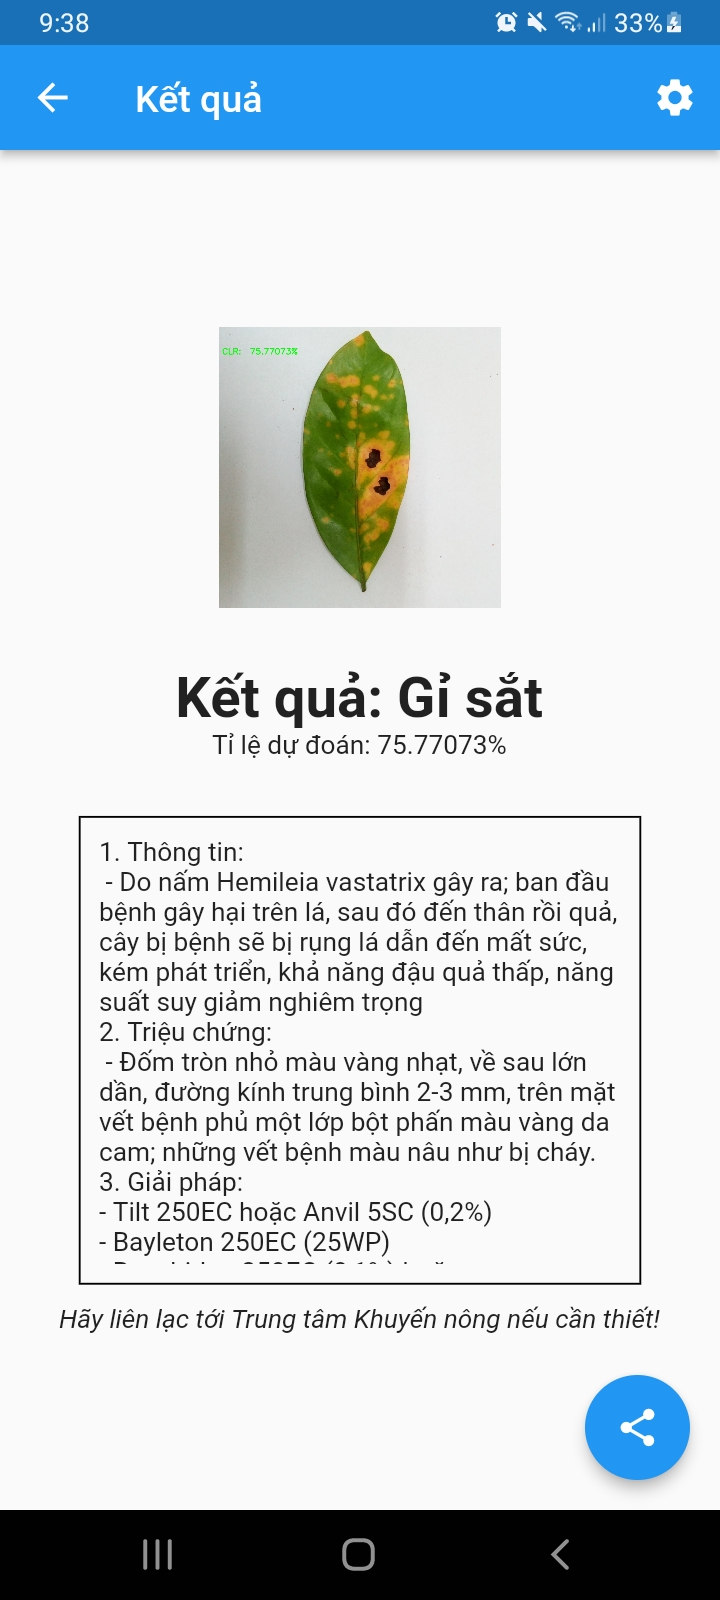
\includegraphics[scale=0.1]{images/screenshot4.jpg}
% 		\caption{Màn hình kết quả}
% 	\end{figure}

% 	Sau khi chờ máy chủ xử lý xong, kết quả sẽ được trả về. Thông tin trả về bao gồm tên sâu bệnh, triệu chứng, một vài thông tin và một vài thuốc chữa. Ở góc phải dưới của màn hình, có nút \textbf{Chia sẻ} qua các ứng dụng, mạng xã hội hay e-mail, để bà con có thể liên lạc tới các Trung tâm về nông nghiệp để được tư vấn thêm.

% 	\begin{figure}[H]
% 		\centering
% 		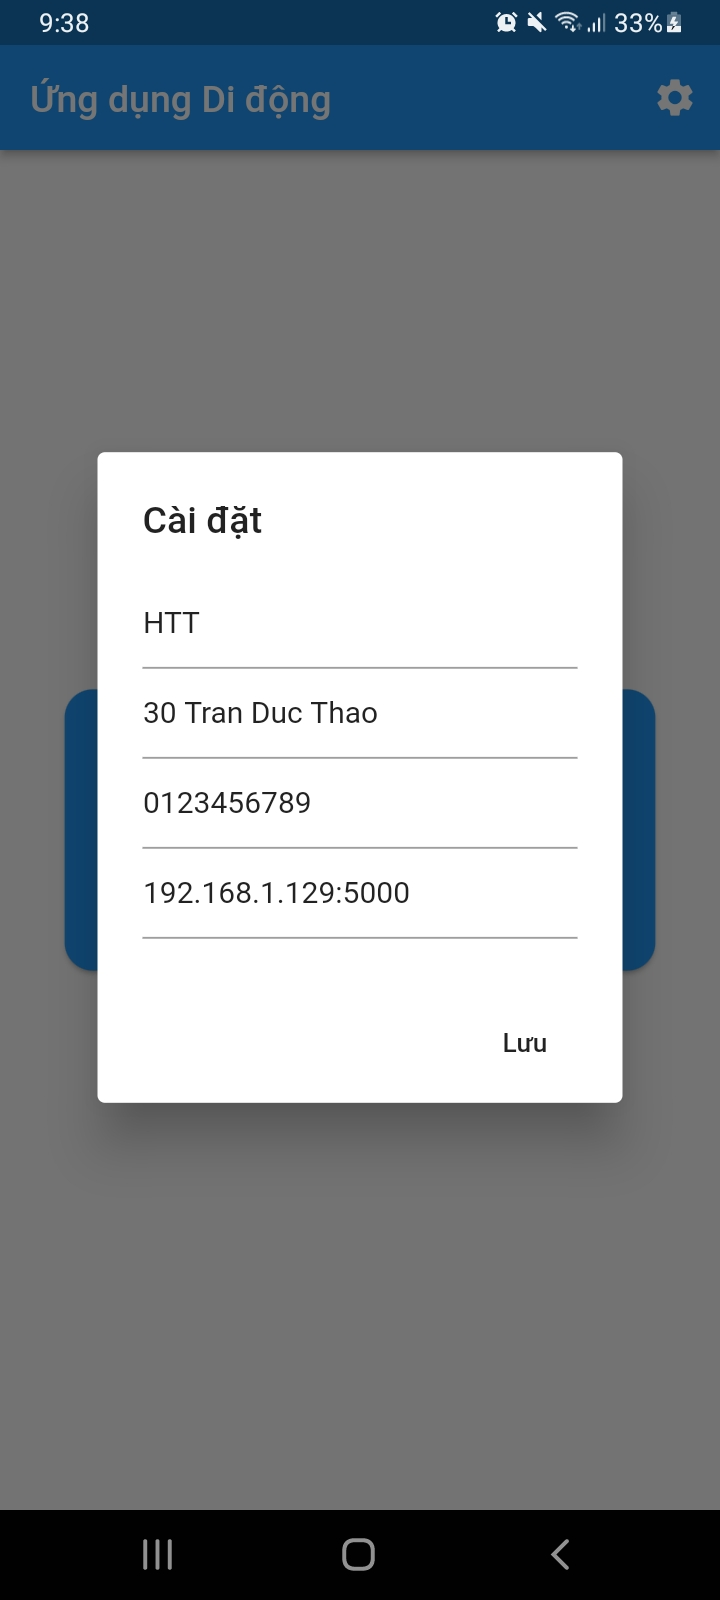
\includegraphics[scale=0.1]{images/screenshot2.jpg}
% 		\caption{Cài đặt}
% 	\end{figure}

% 	Nút \textbf{Cài đặt} có hình bánh răng cưa, ở góc phải trên ở mọi màn hình. Người dùng có thể nhập Tên, Địa chỉ, Số điện thoại để được đính kèm khi \textbf{Chia sẻ} ở Màn hình Kết quả.

% 	\begin{figure}[H]
% 		\centering
% 		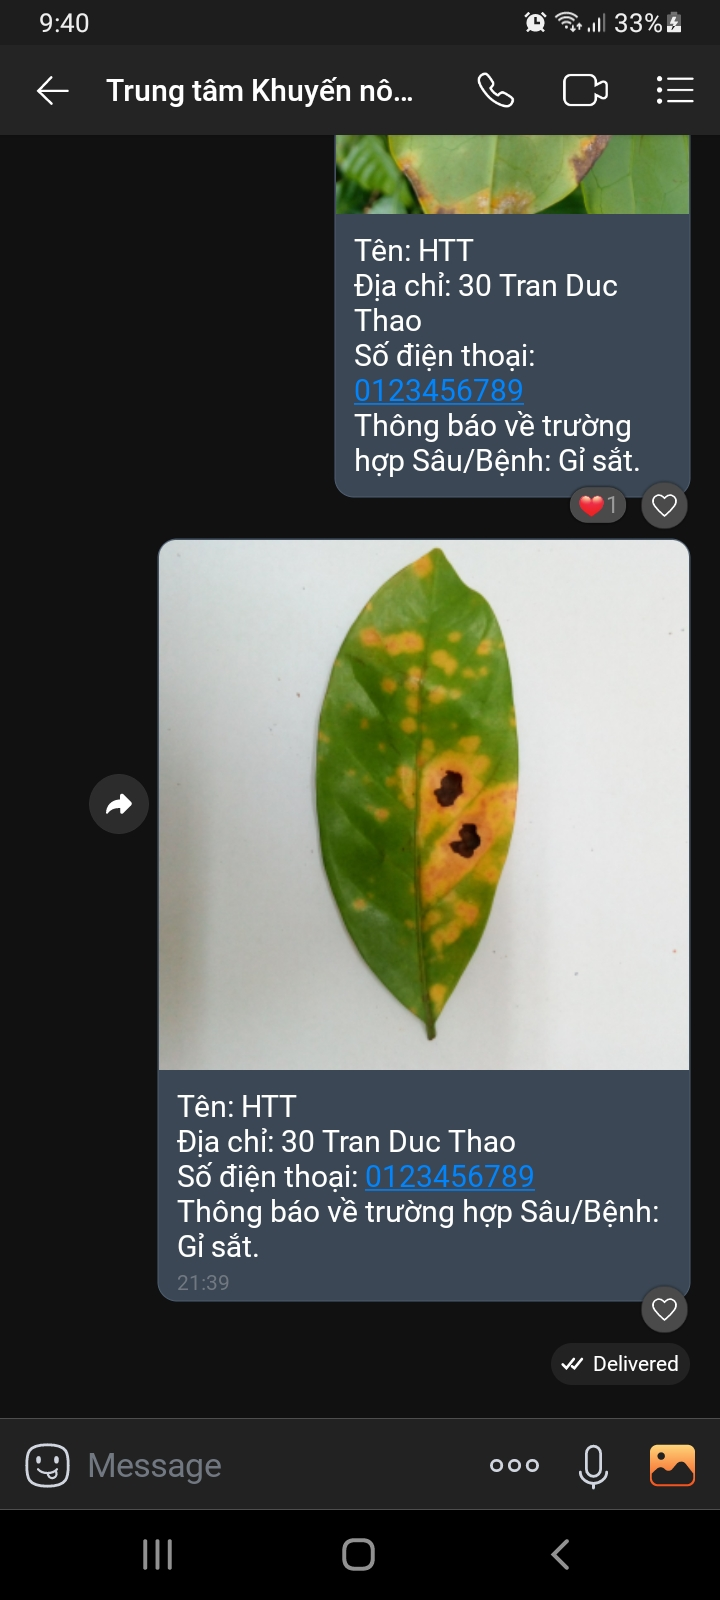
\includegraphics[scale=0.14]{images/screenshot5.jpg}
% 		\caption{Chia sẻ qua các ứng dụng khác (ứng dụng trong ảnh là Zalo)}
% 	\end{figure}
